\documentclass{article}
\usepackage{graphicx}
\usepackage{amsmath, amsthm, amssymb, amsfonts, amsbsy}

\begin{document}
\section{Methods}
For millennia, humans (and other animals) have tried to understand the rules that govern the phenomena surrounding them based on observations. This knowledge allowed for prediction and inventions that improved their way of living, such as empirical laws in any field of fundamental science and consequently applied science. In the last 5 decades, with the advent of several kinds of sensors, fast electronics and large storage capacity, observations have become more and more numerous with a great level of detail (the "deluge of data") and it appears that this way of learning has become more necessary in the present than ever before.

Datasets became very large in the number of elements as well as very high in its dimensionality (the "Deluge of Data"), in a such way that they are no longer amenable for a human operator to analyze them. To be able to deal with this problem, researchers and engineers started using computers in particular methods of Machine Learning. Machine Learning is a subfield of computer science that studies and develops algorithms meant to find new structures or rules a given experiment or phenomenon is based on. Arthur Samuel defined machine learning as a "Field of study that gives computers the ability to learn without being explicitly programmed" (reference Phil Simon (March 18, 2013). Too Big to Ignore: The Business Case for Big Data. Wiley. p.89. ISBN 978-1-118-63817-0.)

However, conventional machine learning techniques required careful and domain-specific design in order to achieve good results. For examples, it would required a considerable amount expertise of the phenomenon to determine an algorithm and/or model that would a good approximation of what was actually happening in the experiment under study.

In this context, a dataset consists of m points (examples) on a n-dimensional space (input space). If to each input there exists an extra object representing the “true” value that the experiment output, the dataset is said to be labeled otherwise it is unlabeled. 

The most commonly used form of machine learning uses labeled datasets. This is called supervised learning.

\subsection{Supervised Learning}
\label{subsec:supervised-learning}
These algorithms are fed some dataset that was the input of the experiment. 

In labeled datasets, each sample (n-dimensional) has attached a “right answer”. Algorithms that receive such an input data are called supervised learning algorithms. These algorithms are usually iterative methods. In this situation, the method modifies itself to output the best possible answer. This modification follows a set of operations (called the training algorithm) that depend on some measure of dissimilarity between the outputs of the model in the current configuration and the corresponding labels. This function (often thought of as a distance) is called the loss function. Examples of loss functions are Mean-Squared Error of Cross Entropy. In each iteration, the training algorithm will calculate the necessary adjustments in order to the loss function smaller. After a certain number of iterations, the algorithm will, possibly, converge on a solution that is a good enough approximation of the experiment under consideration.

In machine learning, we must choose a model (or framework) to work with. In the case of linear regression, the output of the algorithm is a linear function of the form $y = mX + b$, where m and b are the adjustable parameters. This choice strongly conditions the power of the algorithm. If, for instance, y depends on $X$ quadratically, linear regression may not yield the best results; however, depending on the situation it may provide a good enough approximation.
Another choice the user must define a priori is the training algorithm. A simple example of such an algorithms is gradient descent. 

When using this methods, we may not only be interested in explaining the data we have but also predict the outcome of the experiment in untested situations. 


More formally, the computer receives a number, m, of examples of input as a (n-dimensional) feature vectors $\vec{x_i}, i = 1,2, \ldots ,m$ and corresponding (p-dimensional) target (“true”) value $\vec{ y_i}, i=1,2, \ldots ,m$ and tries to find the element in the family of functions (hypothesis class) $h_{\theta}$ parameterized by $\theta$ such that $\vec{ y_i}  \approx h_\theta \left(\vec {x_i} \right)$ for each example. 

\subsubsection{Linear Regression}
\label{subsubsec:linear-regression}
In the context of linear regression, we restrict ourselves to a family of function such that:
\begin{equation}
h_{\vec{\theta},b} ( \vec{x} ) = \sum_{j = 1}^{m} \theta_j x_j + b = \theta \cdot \vec{x} + b
\end{equation}
where $\theta$ and $b$ are the parameters to be learnt.

A common choice for the loss function is the Mean Squared Error (MSE), defined as:

\begin{equation}
J \left( \theta , b\right) = \frac{1}{2} \sum_{j=1}^m \left[ h_{\theta,b} \left( \vec{x}^{(j)} \right) -  y^{(j)} \right]^2 =  \frac{1}{2} \sum_{j=1}^m \left( \theta \cdot \vec{x}^{(j)} + b - y ^{(j)} \right) ^2
\label{eq:MSE-definition}
\end{equation}

Most training algorithms require the knowledge of the gradient of the loss function with respect to the model's parameters to determine the update rule. In this situation, the gradient would be:

\begin{eqnarray}
\frac{ \partial J}{\partial \theta_i } &=& \sum _{j= 1}^m x_i^{(j)} (  h_{\theta, b} ( x^{(j)}) - y^{(j)} ) \\
\frac{ \partial J}{\partial b } &=&  \sum _{j= 1}^m (  h_{\vec{\theta}, b} ( x^{(j)}) - y^{(j)} )
\label{eq:MSE-gradient}
\end{eqnarray}

And the parameters would be updated as:
\begin{eqnarray}
\theta_i^{n+1} &=& \theta_i^{n} - \eta \left[\nabla_{\theta} J(\theta^n,b^n )\right]_i \\
b^{n+1} &=& b^n - \eta \frac{\partial J}{\partial b} \left(\theta^n,b^n \right)
\label{eq:GD-update-rule}
\end{eqnarray}
where $\eta$ is the learning rate defined by the user.


\subsubsection{Logistic Regression}
\label{subsubsec:Logistic-Regression}
Many times, machine learning is used to perform a classification task, i.e., trying to assign a class (discrete value) to some input vector. For instance, we could apply linear regression and set a  threshold value to define the boundary between two class. However this method is very sensitive to extreme value of the input. In the case of binary classification $y^{(i)}$ can only be either 1 or 0. In this situation Logistic Regression is usual a better choice. With logistic regression we try to find the predictor choosing a different hypothesis class: 
\begin{equation}
h_{ \theta, b } (x) = \sigma ( \theta \cdot x + b) = \frac{1}{ 1 + exp(-\theta \cdot x - b) }
\label{def:logistic-regression}
\end{equation}
Note that this function (called the sigmoid function or logistic function) is a continuous for all values of $x$. It is always positive, monotonically increasing from zero to one. This leads to the interpretation of the output of the logistic regression as the probability of the class labeled as “1” happening given the input vector x: 
\begin{eqnarray}
P( Y=1 \mid  X = x ) &=& \frac{1}{ 1 + \exp(-\theta \cdot x - b)} \leqslant 1 \\
P( Y=0 \mid  X = x ) &=& 1 - P( Y=1 \mid  X = x )
\end{eqnarray}

The cost function in this case is usually defined as:
\begin{equation}
J(\theta,b) = - \sum _{j= 1}^m ( y^{(j)} \log(h_{\theta,b}(x^{(j)})) + (1-y^{(j)}) \log(1- h_{\theta,b}(x^{(j)})) )
\end{equation}

Since in this setup $y^{(j)}$ can only be either 1 or 0, only one of the terms inside the summation is non-zero.

The gradient of this loss function is:
\begin{equation}
\nabla _{\theta,b} J(\theta,b) = \sum _{j= 1}^m x^{(j)} ( h_{\theta,b}(x^{(j)}) - y^{(j)} )
\end{equation}

A generalization of the logistic regression to a many-classes situation is the Softmax Regression, where the probabilistic interpretation is applied.

In classification task, we are looking for the boundary between classes in the feature space. The techniques I talked above can only resolve problems in which the classes are linearly separable (where the boundary is an hyper-plane in the feature space). But this is not always the case. Sometimes the region corresponding to a particular class may even be disjoint. In such case linear classifiers are not powerful enough to solve the problem. (As an example consider the Exclusive OR function where the inputs are two binary valued variables. There is not straight line in the input space that separates the class “0” and the class “1”.)

\subsection{Artificial Neural Networks}
\label{subsec:ANN}

A much more powerful concept is that of Artificial Neural Networks. 
An artificial neuron (hereafter neuron unless stated otherwise) is a computational unit that takes as input the vector $x$ and outputs
\begin{equation}
h_{w,b} (x) = f\left( w \cdot x + b \right) = f \left( \sum_{i=1}^n w_i x_i + b  \right)
\end{equation}

where $f\colon \textbf{R} \rightarrow \textbf{R}$ is called the activation function. The vector $\textbf{w}$ and the value of b (called the bias or intercept term), as before, can be tuned according to some algorithm to perform a designated task as good as possible. 

If the activation function is the sigmoid function we recover the logistic regression.

Another example of activation function is the hyperbolic tangent, which increases from -1 to 1. 
Lately, researchers and engineers have started using the rectified linear function (RELU) particularly in the context of deep neural network (which I'll talker later in this document). This function is defined as
\begin{equation}
RELU(z)= \max(z,0) = 
\begin{cases}
    z,& \text{if } z\geq 0\\
    0,              & \text{if } z < 0
\end{cases}
\end{equation}

This activation function is significantly different from the ones referred before because it is not bounded as $z$ increases. Moreover, it is not differentiable when $z=0$ although this doesn't become a problem in practice because it is differentiable at any point arbitrarily close to 0.

A Artificial Neural Network (ANN) is put together by hooking together many of these simple neurons by means of function composition where the output of one neuron is the input of another.


\begin{figure}[!h]
	\centering
	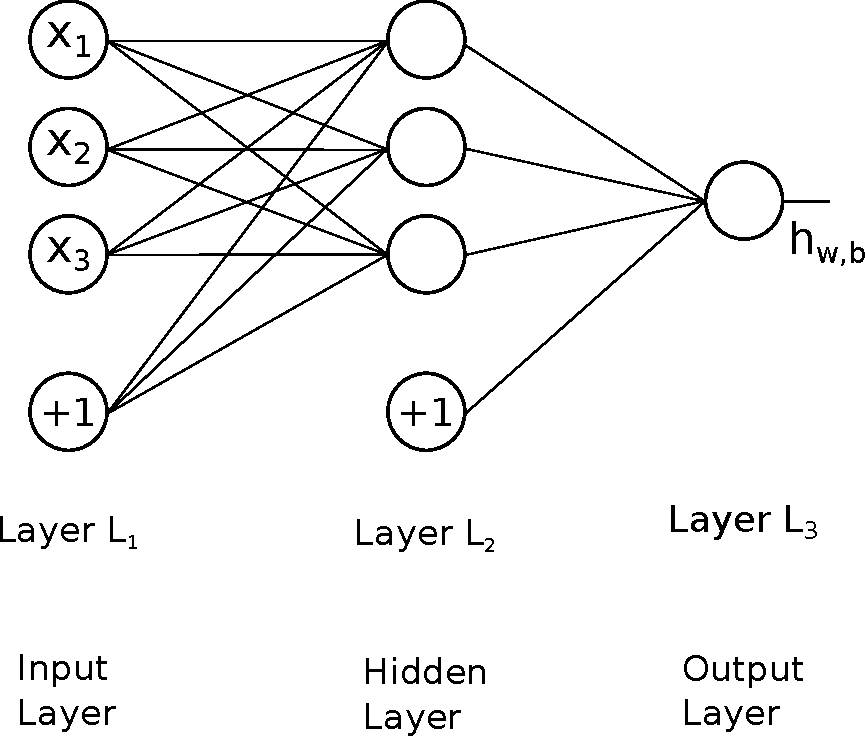
\includegraphics[width=\linewidth]{firstANN.pdf}
	\caption{Graphical visualization of an illustrative example of an artificial neural network. This ANN is composed by three layers with three neurons on the first two and one neuron on the output layer. The connections between all the neurons are also represented, in addition to the connection to the bias term represented by the extra nodes on the bottom with the label "+1".
}
\label{fig:first-ANN}
\end{figure}
In the Fig. \ref{fig:first-ANN} is a graphical representation of what was just mentioned. On the left, we have the input layer (layer $L_1$) where the input vector $(x_1,x_2,x_3)$ is fed. In the middle there are three neurons. These are called hidden neurons and they compose one hidden layer ($L_2$). Finally, there is the output layer with only one neuron. There are also two nodes on the bottom that represent the bias term.

In this example, there are connections between all neurons of one layer to the neurons in the next layer. This ANN is said to be fully connected (or densely connected). For each connection there is an associated parameter (weight) and also a bias parameter. The input of each neurons in the hidden layer is a linear combination of the output of the neurons in the previous layer weighted by the parameters of the corresponding connections and summed with the bias term. In this case, the weights for the connections coming in to the first neuron in the layer L2 are $w_{1,1}^{(1)},w_{1,2}^{(1)},w_{1,3}^{(1)}, b_1^{( 1 )}$ and its input is:
\begin{equation}
z_1^{(2)} = \sum_{i=1}^3 w_{1,i}^{(1)} a_i^{(1)} + b_1^{(1)}
\end{equation}
This input is then fed into the activation function which reveals the outputs of this neuron as 
\begin{equation}
a_1^{( 2 )} = f\left( z_1^{(2)} \right)
\end{equation}

We denoted the number of layer as $n_l$ and the number of neurons in the layer $L_l$ as $S_l$. In the example above $n_l=3$, $S_1 = S_2 = 3$ and $S_3 = 1$

In general, when the network is densely connected, the input of the neuron i in the layer j is:
\begin{equation}
z_i^{(j)} = \sum_{k=1}^{S_{l-1}} w_{i,k}^{(j)} a_k^{(j-1)} + b_i^{(j-1)}  
\end{equation}
And its output is:
\begin{equation}
a_i^{(j)} = f(z_i^{(j)})
\end{equation}
It is also convenient to introduce a matrix notation such that:
\begin{equation}
\textbf{z}^{(j)} = \textbf{W}^{(j)} \textbf{a}^{(j-1)} + \textbf{b}^{(j-1)}
\end{equation}
where the vector $\textbf{z}^{(j)}$, $\textbf{a}^{(j)}$ and $\textbf{b}^{(j)}$ represent the input, output and bias parameter of all neurons in Layer $L_j$

The output of the output layer is denoted $\textbf{h}_{\textbf{W},\textbf{b}}\left( \cdot \right) = \textbf{a}^{(L)}\left( \cdot \right)$



With this concept of Artificial Neural Network, we now have a much more framework to create models that can be trained to compute much more complex function than the ones computable with traditional machine learning algorithms.
 
There's still the need to define the training algorithm. To utilize the usual gradient descent, it is necessary to compute the gradients of the loss function with respect to all the adjustable parameter of ANN. These gradients are usually computed using the back-propagating algorithm. In this method, the label is subtracted from the output value as an estimate of the gradient on the output layer. This value is then propagated backwards layer by layer applying the chain rule for derivatives, which will depend on the chosen activation functions. With the gradients estimated, the parameters are update in the way defined earlier in equation \ref{eq:GD-update-rule}

The key aspect of learning with ANN is that, due to its generalization power, the output functions are not designed by a human: they are learned from the data.

But this framework leads to question of how to define the model. In other words, how to define the architecture of the ANN, i.e., how many neurons should there be in the ANN and should they be connected? There are two basic topologies: shallow networks and deep networks. In shallow networks, there is at most one hidden layer, whereas a network is said to be deep if it has two or more hidden layers. This distinction has become very important over the last three decades. On the one hand, it has been shown that a shallow ANN with only one arbitrarily large hidden layer could approximate a function to any level of precision (REFERENCE Horniket al.,1989). Nonetheless, this level of precision would only increase with exponentially increasing number of neurons, becoming computationally very demanding. On the other hand, deep neural networks are conceptually more interesting because each layer can be thought of as representation of the input in higher and higher level of abstraction, approaching the way humans perceive the world. However with the back-propagation and gradient descent with the usual sigmoid or tanh function one could easily reach the problem of “the vanishing gradients”, when the activation function saturated and the training wouldn't go any further. Moreover, even in cases when training was possible deep networks were found to perform worse than shallow networks.

However, in the past decade there have been several theoretical and technological advances that brought deep neural network back to live.

\subsection{Deep Learning}
\label{subsec:Deep-Learning}
Representation learning is a family of methods that allow machines to find new ways of representing the raw data it was fed with. Deep Learning tries to accomplish this in a "layer by layer" manner. In a deep neural network, each layer holds a new representation of the input data, by transforming the output of the previous layer into a new representation that is more abstract. Composing many of these layer, it should be possible to extract very complex function can be learnt. For the case of classification task, higher layers of representation may amplify aspects of the input that are important for the discrimination and suppress irrelevant features.
\end{document}